\documentclass[11pt, oneside]{article}   	% use "amsart" instead of "article" for AMSLaTeX format
\usepackage{geometry}                		% See geometry.pdf to learn the layout options. There are lots.
\geometry{letterpaper}                   		% ... or a4paper or a5paper or ... 
%\geometry{landscape}                		% Activate for rotated page geometry
\usepackage[parfill]{parskip}    			% Activate to begin paragraphs with an empty line rather than an indent
\usepackage{graphicx}				% Use pdf, png, jpg, or eps§ with pdflatex; use eps in DVI mode
								% TeX will automatically convert eps --> pdf in pdflatex		
\usepackage{amssymb}
\usepackage{hyperref}
\usepackage{amsmath}
\usepackage{listings}
\usepackage{mathtools}
\usepackage{enumerate}
\usepackage{tikz}
\usepackage{algorithm}   
\usepackage{algpseudocode} 
\newcommand{\ck}[1]{\textcolor{cyan}{CK: #1}}
\newcommand{\jc}[1]{\textcolor{orange}{JC: #1}}
\newcommand{\hm}[1]{\textcolor{blue}{HM: #1}}

\title{Homework 2 \\ CSC 277 / 477 \\ End-to-end Deep Learning \\ Fall 2024}
\author{Henry Yin - \texttt{hyi1n2@u.rochester.edu}}
\date{}					


\begin{document}

\maketitle

\begin{center}
    \textbf{Deadline:} 10/18/2024
\end{center}


\section*{Instructions}

Your homework solution must be typed and prepared in \LaTeX. It must be output to PDF format. To use \LaTeX, we suggest using \url{http://overleaf.com}, which is free.

Your submission must cite any references used (including articles, books, code, websites, and personal communications).  All solutions must be written in your own words, and you must program the algorithms yourself. \textbf{If you do work with others, you must list the people you worked with.} Submit your solutions as a PDF to Blackboard. 


Your programs must be written in Python. The relevant code should be in the PDF you turn in. If a problem involves programming, then the code should be shown as part of the solution. One easy way to do this in \LaTeX \, is to use the verbatim environment, i.e., \textbackslash begin\{verbatim\} YOUR CODE \textbackslash end\{verbatim\}.



%%%%%%%%%%%%%%%%%%%%%%%%%%%%%%%%%%%%%%%%%%%%%




%CodeCogs: \url{https://www.codecogs.com/latex/eqneditor.php}

%MathType: \url{http://www.dessci.com/en/products/mathtype/}
%For MathType, you have to tell it to export as LaTex. 


\clearpage

% \section*{Problem ? - Prompt Engineering}


\section*{Problem 1 - LoRA (22 Points)}
Fine-tuning large pre-trained language models for downstream tasks is common in NLP but can be computationally expensive due to the need to update all model parameters. LoRA (LOw-Rank Adaptation) offers a more efficient alternative by only adjusting low-rank components instead of the full parameter set.

Specifically, for a pre-trained weight matrix $W_0\in \mathbb{R}^{d\times k}$, the model update is represented with a low-rank decomposition $W_0+\Delta W=W_0+BA$, where $B\in \mathbb{R}^{d\times r}, A\in \mathbb{R}^{r\times k}$, and the rank $r \ll \min(d,k)$.
During training, $W_0$ is frozen, while $A$ and $B$ are trainable. For $h = W_0x$, the modified forward pass yields: $h = W_0 x + \Delta W x = W_0 x + BA x$, as shown in Fig.~\ref{fig:lora}.
In this problem, you'll fine-tune a pre-trained language model using LoRA for sentiment classification. 

\begin{figure}[h]
    \centering
    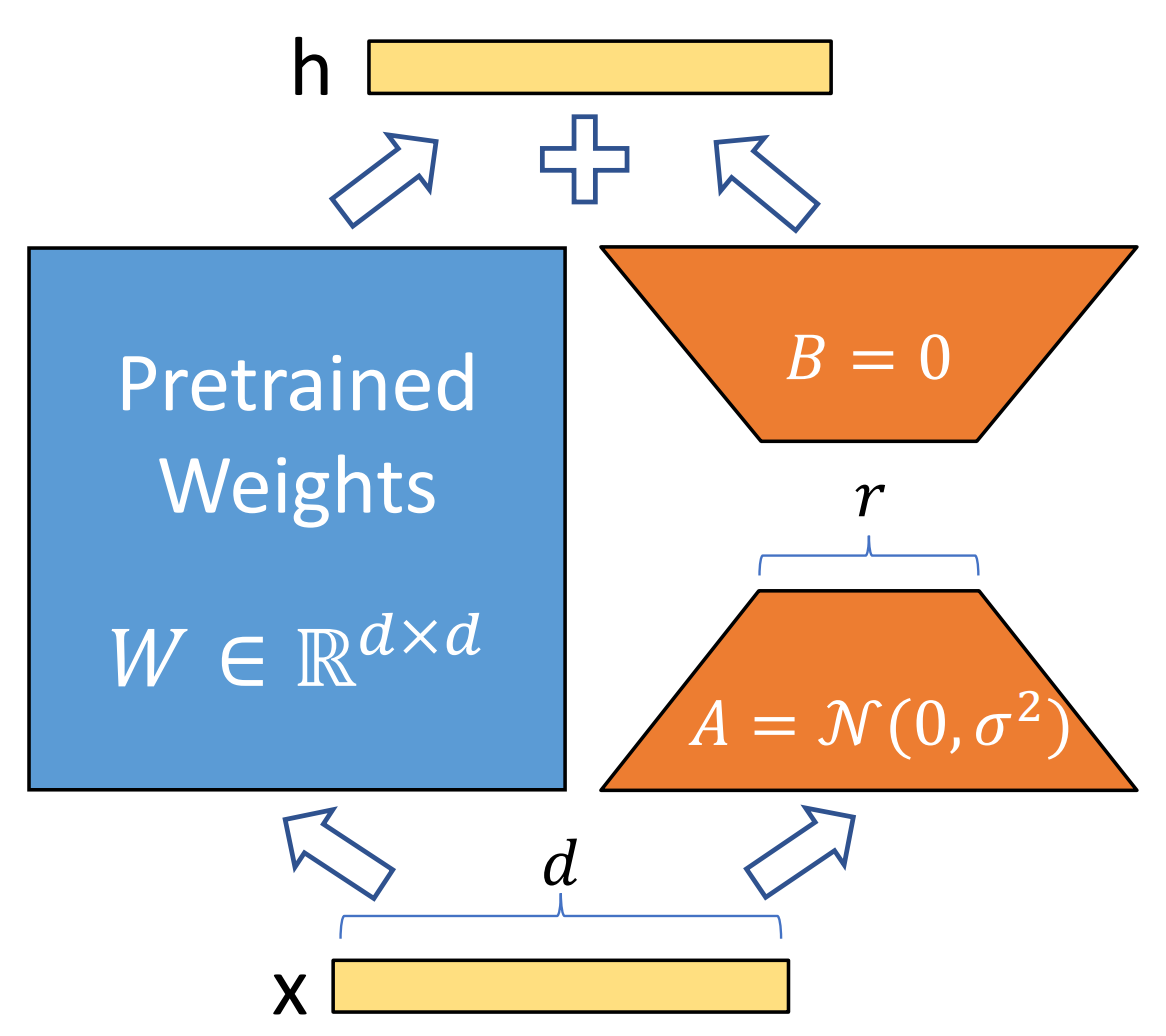
\includegraphics[width=0.35\textwidth]{images/lora.png}
    \caption{
    Illustration of \href{https://arxiv.org/pdf/2106.09685.pdf}{LoRA}. Only $A$ and $B$ are trainable.
    }
    \label{fig:lora}
\end{figure}


\subsection*{Part 1: Understanding LoRA}
\subsubsection*{Part 1.1: Analyzing Trainable Parameters (2 Points)}
Given the description, determine the ratio of trainable parameters to the total parameters when applying LoRA to a weight matrix $W_0\in \mathbb{R}^{d\times k}$ with the following dimensions: $d = 1024$, $k = 1024$, and a low-rank approximation of $r = 8$. \\
\textbf{Deliverable:}
Provide the formula/expression for this ratio.

\textbf{Answer:} \\
Total parameters in the original weight matrix $W_0$ is:
\[ \text{Total Parameters} = d \times k = 1024 \times 1024 = 1,048,576 \]
\\
LoRA introduces low rank decomposition where the original weight matrix $W_0$ is approximated by to smaller matrices.
One with size \( W_A \in \mathbb{R}^{d \times r} \) and one of size \( W_B \in \mathbb{R}^{r \times k} \).
\\
The number of trainable parameters in LoRA then:
\[ \text{Trainable Parameters} = (d \times r) + (r \times k) = (1024 \times 8) + (8 \times 1024) = 8192 + 8192 = 16,384 \]
\[ \frac{\text{Trainable Parameters}}{\text{Total Parameters}} = \frac{16.384}{1,048,576} \approx 0.015625 \]
The ratio of trainable parameters to total parameters is 0.0156 (i.e. $1.56\%$)

\subsubsection*{Part 1.2: LoRA Integration in Transformer Models (2 Points)}
Read the following paragraphs in the \href{https://arxiv.org/abs/2106.09685}{LoRA} paper:
\begin{itemize}
    \item \texttt{Section 1 - Introduction}; specifically \texttt{Terminologies and Conventions}
    \item \texttt{Section 4.2 - Applying LoRA to Transformer}
    \item \texttt{Section 5.1 - Baselines}; specifically \texttt{LoRA.}
\end{itemize}
\textbf{Question:}
For a Transformer architecture model, where is LoRA typically injected? (Options: query/key/value/output projection matrices)

\textbf{Answer:} \\
\textit{Query and Value} projection matrices.

\subsection*{Part 2:  Fine-Tuning for Sentiment Classification}
\subsubsection*{Part 2.1: Fine-Tuning Without LoRA (6 Points)}
\href{https://huggingface.co/}{Hugging Face} provides a user-friendly framework for natural language processing tasks. If you haven't used it before, this is a great opportunity to get familiar with it. 

\begin{enumerate}
    \item Follow the \href{https://huggingface.co/docs/transformers/training}{Hugging Face fine-tuning tutorial} and install the necessary packages to set up the components required for training: \texttt{transformers} (required), \texttt{datasets}(required), and \texttt{evaluate} (optional, depending on your implementation).
    \item Fine-tune the \texttt{\href{https://huggingface.co/roberta-base}{roberta-base}} model on the Tweet Eval Sentiment dataset. Make sure to set the \texttt{num\_labels} parameter correctly. You can load the dataset using: \texttt{datasets.load\_dataset("tweet\_eval", name="sentiment")}.
    \item For training settings, fine-tune the model for \textbf{1 epoch} using \href{https://huggingface.co/docs/transformers/training#trainer}{Hugging Face's PyTorch Trainer}. Default parameters like learning rate can be used. For batch size, adjust based on your computational resources. Estimated computational cost with a batch size of $16$: GPU memory of 6.6 G and runtime within 10 Min. CPU runtime: 1 H.
    
    \item \label{step4} Record the following metrics: \textbf{(a)} Number of \textit{total} and \textit{trainable} parameters;  \textbf{(b)} Training time; \textbf{(c)} GPU memory usage during training (optional but encouraged); \textbf{(d)} Performance on the test set (Accuracy, F1 score, and loss).

    If implemented correctly, the accuracy score on the test set should be above $0.6$.
\end{enumerate}
\textbf{Deliverable:}
\begin{enumerate}
    \item Recorded metrics as described in Step 4 in \LaTeX~table(s).
    \item Your code implementation.
\end{enumerate}

\textbf{Answer:} \\
\begin{center}
    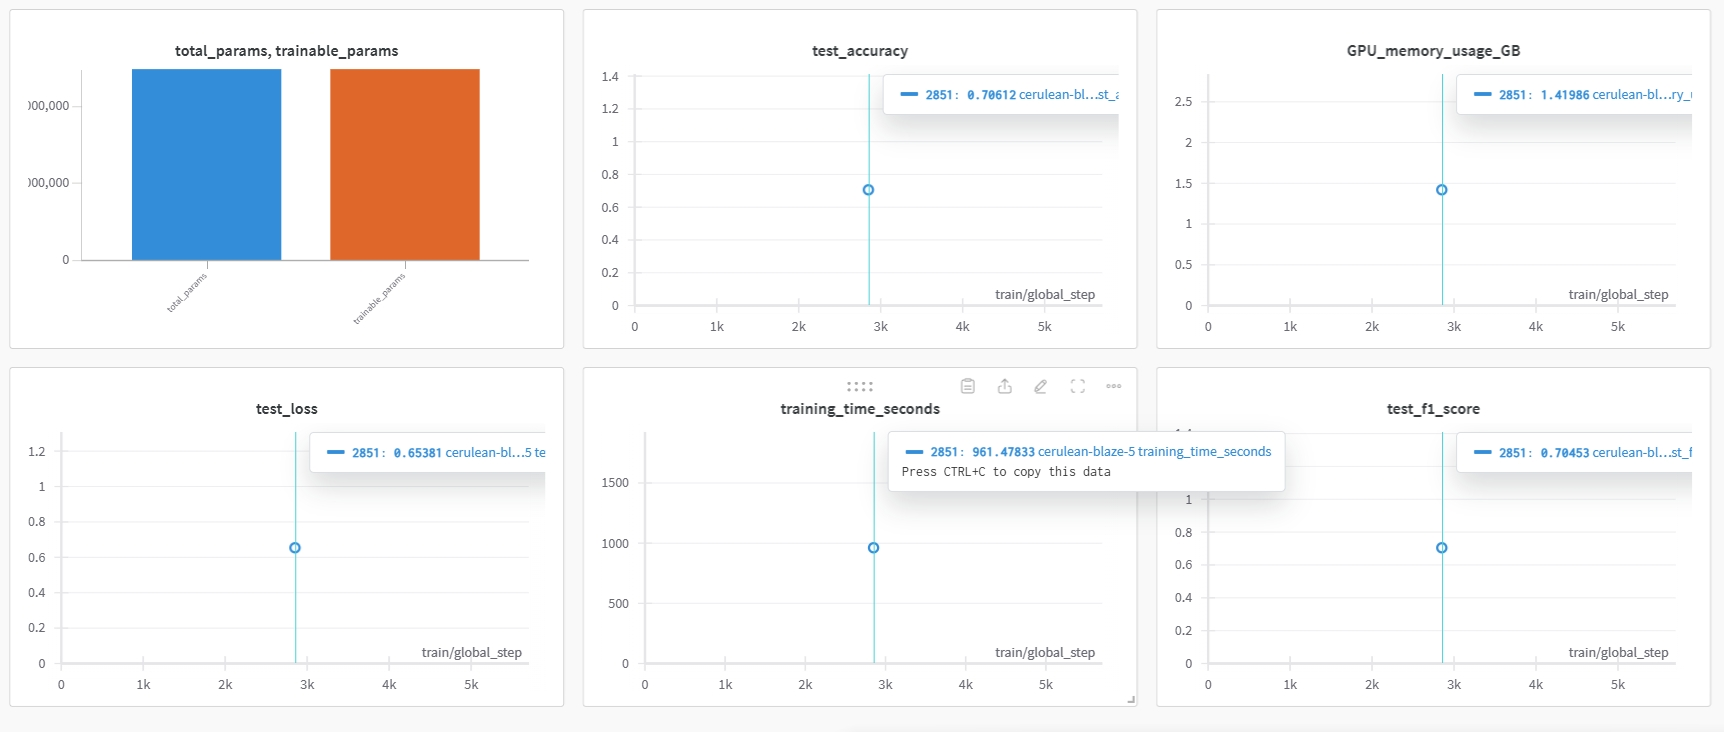
\includegraphics[width=\textwidth]{p1p2_pic/RoberTaFT.png}
\end{center}
\\
NOTE: There are 124,647,939 Total Parameters In the Model.
\\
\textbf{Code Implementation: }
\begin{verbatim}
import time
import torch
import wandb
from datasets import load_dataset
from transformers import RobertaTokenizer, RobertaForSequenceClassification, Trainer, TrainingArguments
from sklearn.metrics import accuracy_score, f1_score

wandb.init(project="sentiment-classification", config={
    "model": "roberta-base",
    "dataset": "Tweet Eval Sentiment",
    "epochs": 1,
    "batch_size": 16,
})

dataset = load_dataset("tweet_eval", name="sentiment")
tokenizer = RobertaTokenizer.from_pretrained("roberta-base")

def tokenize_function(examples):
    return tokenizer(examples["text"], padding="max_length", truncation=True)

tokenized_datasets = dataset.map(tokenize_function, batched=True)

model = RobertaForSequenceClassification.from_pretrained("roberta-base", num_labels=3)
device = torch.device("cuda" if torch.cuda.is_available() else "cpu")
model.to(device)

# Record total and trainable parameters
total_params = sum(p.numel() for p in model.parameters())
trainable_params = sum(p.numel() for p in model.parameters() if p.requires_grad)
wandb.config.update({
    "total_params": total_params,
    "trainable_params": trainable_params
})

training_args = TrainingArguments(
    output_dir="./results",
    num_train_epochs=1,
    per_device_train_batch_size=16,
    evaluation_strategy="epoch",
    save_strategy="epoch",
    fp16=True, 
    save_total_limit=1,
    load_best_model_at_end=True,
    report_to="wandb",
)

# Define compute_metrics function calculate accuracy and F1 score
def compute_metrics(p):
    preds = p.predictions.argmax(-1)
    accuracy = accuracy_score(p.label_ids, preds)
    f1 = f1_score(p.label_ids, preds, average="weighted")
    return {"accuracy": accuracy, "f1": f1}

trainer = Trainer(
    model=model,
    args=training_args,
    train_dataset=tokenized_datasets["train"],
    eval_dataset=tokenized_datasets["validation"],
    compute_metrics=compute_metrics,
)

start_time = time.time()

trainer.train()

training_time = time.time() - start_time
wandb.log({"training_time_seconds": training_time})

if torch.cuda.is_available():
    allocated_memory = torch.cuda.memory_allocated() / (1024 ** 3)
    reserved_memory = torch.cuda.memory_reserved() / (1024 ** 3)
    max_allocated = torch.cuda.max_memory_allocated() / (1024 ** 3)
    print(f"GPU allocated memory: {allocated_memory:.3f} GB")
    print(f"GPU reserved memory: {reserved_memory:.3f} GB")
    print(f"Max GPU allocated memory: {max_allocated:.3f} GB")


metrics = trainer.evaluate(tokenized_datasets["test"])
wandb.log({
    "test_accuracy": metrics["eval_accuracy"],
    "test_f1_score": metrics["eval_f1"],
    "test_loss": metrics["eval_loss"],
})

wandb.finish()
\end{verbatim}

\newpage

\subsubsection*{Part 2.2: Fine-Tuning With LoRA using PEFT (4 Points)}
The \href{https://github.com/huggingface/peft}{PEFT} (Parameter-Efficient Fine-Tuning) repository provides efficient methods for adapting models, including LoRA, and integrates with Hugging Face. In this section, you’ll fine-tune RoBERTa with LoRA using PEFT.
\begin{enumerate}
    \item Copy your code from Part 2.1 (fine-tuning without LoRA).
    \item \label{step2} Read the \href{https://huggingface.co/docs/peft/quicktour}{PEFT quick tour}. Prepare the model for fine-tuning with LoRA with the following settings: Set the rank to 8; Adjust the \texttt{inference\_mode} and \texttt{task\_type} parameters to appropriate values; Keep all other parameters as default (only adjust the three mentioned).
   \item Apply the same training recipe as in Part 2.1 and fine-tune RoBERTa with LoRA.
\end{enumerate}


\textbf{Deliverable:}
\begin{enumerate}
    \item Recorded Metrics as described in Part 2.1 Step~\ref{step4} in \LaTeX~table(s)
    \item Your code snippet of the implementation of LoRA into the model.
\end{enumerate}

\textbf{Answer:} \\

\subsubsection*{Part 2.3: Comparison and Analysis (3 Points)}

Now that you've fine-tuned the RoBERTa model with and without LoRA, compare their performance using the following criteria:
\begin{enumerate}
    \item \textbf{Efficiency}: Compare total parameters, trainable parameters, GPU memory usage (optional), and training time.
    \item \textbf{Performance}: Compare test set results in terms of accuracy, F1 score, and loss.
    \item Consider other aspects: drawing inspiration from the \href{https://arxiv.org/abs/2106.09685}{LoRA paper} \texttt{Section 4.2 - APPLYING LORA TO TRANSFORMER - Practical Benefits and Limitations.}
\end{enumerate}
\textbf{Deliverable}: Provide concise answers to these three aspects, each with one or two sentences, to summarize your findings and insights.

\textbf{Answer:} \\


\subsubsection*{Part 3: Influence of Model Size (5 Points)}
In this part, you will replicate the experiment from Part 2, but using a much smaller model, \href{https://huggingface.co/huawei-noah/TinyBERT_General_4L_312D}{TinyBERT}. 
Fine-tune the model both with and without LoRA. Simply replace the model name in your previous code, keeping the same training settings and logging metrics. The expected accuracy should exceed $0.50$.

\textbf{Deliverable:}
\begin{enumerate}
    \item Provide the same metrics (with and without LoRA) as in Part 2 in \LaTeX~table(s).
    \item Compare the performance of your models with a naive predictor that always guesses the majority class. Which one is better?
    \item Reflect on your Part 2 analysis. Determine if the same observations apply to this smaller model and discuss factors that could explain differences (if any).
\end{enumerate}

\textbf{Answer:} \\




\section*{Problem 2 - Using Pretrained-Model Embedding (20 Points)}
Pretrained models help transfer knowledge to new tasks by generating meaningful data representations, which can be used for downstream tasks like classification.
In this problem, you'll use pretrained models to generate embeddings for the Visual Question Answering (VQA) task. The task is simplified into a classification problem, where the model must choose the correct answer based on an image and a question. We'll use the DAQUAR dataset, available~\href{https://www.kaggle.com/datasets/tezansahu/processed-daquar-dataset}{here}, but will replace the original files with new versions (\texttt{new\_data\_train.csv}, \texttt{new\_data\_val.csv}, \texttt{new\_data\_test.csv}) that reduce the answer space to 30 classes.

To solve the task, you’ll need two encoders: one for images and one for text. You will explore two setups for extracting embeddings. It's recommended to save these extracted embeddings to avoid repeated computation. If implemented correctly, the test set accuracy is \textbf{at least 0.35}. \textbf{Save the models' test set predictions} for use in Part 3.

\begin{figure*}[h]
    \centering
  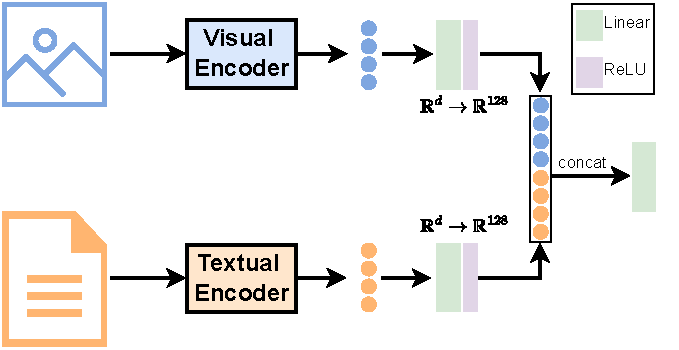
\includegraphics[width=0.6\textwidth]{images/model.pdf}
  \caption{The model architecture.}
  \label{fig:model}
\end{figure*}

\subsection*{Part 1: ResNet + SBERT (7 points)}

Utilize a ResNet-50 model pretrained on ImageNet, to extract image embeddings just \textbf{before} the classification head. Use the sentence transformer \href{https://huggingface.co/sentence-transformers/all-MiniLM-L6-v2}{all-MiniLM-L6-v2} to extract sentence embeddings. Refer to \href{https://huggingface.co/sentence-transformers/all-MiniLM-L6-v2#usage-sentence-transformers}{this tutorial} for implementation.

Implement the model as shown in Fig.~\ref{fig:model}. The model involves a linear layer with ReLU activation for dimension reduction, followed by the concatenation of the processed embeddings. Finally, this concatenated representation is passed through a linear classifier. Train the model and evaluate its performance on the test set. 

\textbf{Deliverable:} \textbf{(a)} Dimensions of the embeddings; \textbf{(b)} Experimental result; \textbf{(c)} Code implementation.

\textbf{Answer:} \\


\subsection*{Part 2: CLIP (7 points)}
 Use the CLIP model (ViT-B/32)'s visual and textual encoder to extract the required embeddings. Refer to its official implementation details \href{https://github.com/openai/CLIP}{here}. Similarly, implement and train the model, then report: \textbf{(a)} Dimensions of the embeddings; \textbf{(b)} Experimental result; \textbf{(c)} Code implementation.

\textbf{Answer:} \\

\subsection*{Part 3: Comparison and Analysis (6 points)}

Analyze the pattern of the questions in the DAQUAR dataset. Review Section 3 and Table 1 of \href{https://openaccess.thecvf.com/content_ICCV_2017/papers/Kafle_An_Analysis_of_ICCV_2017_paper.pdf}{this paper}. Determine how many types of questions DAQUAR (the subset used in this question) is composed of based on the paper's definition. Then divide DAQUAR by question types and analyze and compare the results from both approaches. Discuss potential reasons for any observed differences, considering factors such as the pertaining schedule and their suitability for feature extraction.

\noindent\textbf{Deliverable:}
\begin{itemize}
\item A table containing question types and the number of samples for each type in the dataset (training, validation, and test set).
\item Accuracy scores of both models on the entire test set and for each question type.
\item A comparison of both models for each question type and your analysis.
\end{itemize}


\textbf{Answer:} \\

% \subsection*{\textcolor{red}{Part 4: Comparison with LLM} (6 points)}

 

\section*{Problem 3: Prompt Engineering Techniques (10 Points)}

In this problem, you will experiment with different prompt styles to see how they affect the outputs of a pre-trained Microsoft Phi-1.5 model.

\subsection*{Background}
Prompt engineering is an important skill when working with language models. Depending on how you ask a model to perform a task, the quality of the result can change. In this problem, you'll work with \href{https://huggingface.co/docs/transformers/main_classes/pipelines}{Hugging Face’s transformers library} and apply different prompts to a fact checking task.

\subsection*{Microsoft Phi-1.5 Model}
The Microsoft Phi-1.5 model is designed to be efficient and powerful for a variety of tasks, including text generation and prompt-based learning. Phi-1.5 is known for its smaller architecture, which enables quicker responses while still maintaining the ability to perform well across many tasks. You can find more information about the Phi-1.5 model \href{https://huggingface.co/microsoft/phi-1_5}{on this page}. 

In this problem, you will experiment with three prompt styles:
\begin{enumerate}
    \item \textbf{Short and Direct}: Minimal instructions provided to the model.
    \item \textbf{Few-Shot Learning}: The model is provided with labeled examples before classifying the target text.
\end{enumerate}

\subsection*{Part 3.1: Testing Prompt Variations (5 Points)}

Use the following sentences and test two of your own sentences for sentiment classification:

\begin{itemize}
    \item ``The Great Pyramid of Giza is located in Egypt."
    \item ``4 + 4 = 16."
    \item ``Mount Everest is the tallest mountain on Earth."
    \item ``Bats are blind."
    \item ``Sharks are mammals."
\end{itemize}

Now, add two of your own sentences for testing.

\textbf{Prompts}:
\begin{itemize}
    \item \textbf{Short and Direct}: “Classify the sentiment as positive or negative: [text].”
    \item \textbf{Few-Shot Learning}: 
    \begin{verbatim}
    Statement: "The moon is made of cheese."
    Answer: False
    Statement: "The Eiffel Tower is located in Paris."
    Answer: True
    [text] 
    Answer:
    \end{verbatim}
\end{itemize}

\textbf{Deliverables}:
\begin{itemize}
    \item Run the provided Python code in the separate file \texttt{problem\_3.py} and test the two prompt strategies on each of the five given texts plus two sentences of your own.
    \item Provide outputs.
    \item Summarize how the structure of the prompt affected the model’s responses. Compare the outputs for the different prompt styles and explain the differences.
\end{itemize}

\subsection*{Provided Code}
You will use the Python code provided in the file \texttt{problem\_3.py} to complete the task. Make sure to modify the sentences and experiment with the different prompt styles as described.

\subsection*{Part 3.2: Advanced Prompt Engineering (5 Points)}

In this part, you will experiment with a more advanced prompt engineering technique: \textbf{Expert Prompting}. This technique asks the model to assume the role of an expert or a knowledgeable entity while performing the task. You will compare this approach to the simpler prompt styles used in Part 3.1.

\textbf{Prompts for Expert Prompting}:
\begin{itemize}
    \item \textbf{Expert Prompting}: “You are a world-renowned fact-checker. Please carefully verify the following statement and explain whether it is true or false in detail: [text].”
\end{itemize}

Use the same sentences you used in Part 3.1

\textbf{Deliverables}:
\begin{itemize}
    \item Run the Expert Prompting example on each sentence and compare the results to the output from Part 3.1 (Short and Direct and Few-Shot Learning).
    \item Provide the modified python code and outputs.
    \item Discuss whether the Expert Prompting technique improved the quality of the model’s sentiment analysis. Did giving the model an ``expert personality" help generate more coherent or accurate responses?
\end{itemize}

\textbf{Useful Links:}
\begin{itemize}
    \item Microsoft Phi-1.5 Model: \href{https://huggingface.co/microsoft/phi-1_5}{https://huggingface.co/microsoft/phi-1\_5}
    \item Hugging Face Pipelines: \href{https://huggingface.co/docs/transformers/main_classes/pipelines}{https://huggingface.co/docs/transformers/main\_classes/pipelines}
\end{itemize}





\end{document}   